%%%%%%%%%%%%%%%%%%%%%%%%%%%%%%%%%%%%%%%%%
% Beamer Presentation
% LaTeX Template
% Version 1.0 (10/11/12)
%
% This template has been downloaded from:
% http://www.LaTeXTemplates.com
%
% License:
% CC BY-NC-SA 3.0 (http://creativecommons.org/licenses/by-nc-sa/3.0/)
%
%%%%%%%%%%%%%%%%%%%%%%%%%%%%%%%%%%%%%%%%%

%----------------------------------------------------------------------------------------
%	PACKAGES AND THEMES
%----------------------------------------------------------------------------------------

\documentclass{beamer}

\mode<presentation> {
\usetheme{default} %
\usecolortheme{seagull} 
}

\usepackage{graphicx} % Allows including images
\usepackage{booktabs} % Allows the use of \toprule, \midrule and \bottomrule in tables
\usepackage{tipa}
\usepackage[T1]{fontenc}
\usepackage{tikz}
\usepackage{tabularx}
	\newcolumntype{L}{>{\raggedright\arraybackslash}X}

\pgfdeclareimage[width=\paperwidth]{mybackground}{College.pdf}
%----------------------------------------------------------------------------------------
%	TITLE PAGE
%----------------------------------------------------------------------------------------

\setbeamertemplate{title page}{
        \begin{picture}(0,0)
            \put(-30,-143){%
                \pgfuseimage{mybackground}
            }
            \put(-17,-40.7){%
                \begin{minipage}[b][45mm][t]{226mm}
                    \usebeamerfont{title}{\inserttitle\par}
                \end{minipage}
            }
            \put (-17, -75){%
            	\begin{minipage}[b][45mm][t]{226mm}
			\usebeamerfont{Large}{\insertauthor\par}
			\usebeamerfont{large}{\insertdate\par}
		\end{minipage}
	   }
            \end{picture}
    }

\title[College Scorecard]{Predicting school closings from the DOE College Scorecard} % The short title appears at the bottom of every slide, the full title is only on the title page

\author{Kirsten Regier} % Your name
\date{October 7, 2020} % Date, can be changed to a custom date

\begin{document}

\begin{frame}
\titlepage % Print the title page as the first slide
\end{frame}

%\begin{frame}
%\frametitle{Overview} % Table of contents slide, comment this block out to remove it
%\tableofcontents
%\end{frame}

%----------------------------------------------------------------------------------------
%	PRESENTATION SLIDES
%----------------------------------------------------------------------------------------
%------------------------------------------------
\section{Background} % 1-2 slides
%------------------------------------------------
\begin{frame}
\frametitle{Number of US Postsecondary Institutions}

\begin{figure}
\begin{center}
\includegraphics[width=4.5in]{NCESFastFactsPies2.png}
\caption{Distribution of US colleges by degree type for AY 2012-13 (left) and 2016-2017 (right).  \newline
\tiny{Source: U.S. Department of Education, National Center for Education Statistics. (2019). Digest of Education Statistics, 2018 (NCES 2020-009), Chapter 2., https://nces.ed.gov/fastfacts/display.asp?id=84}}
\end{center}
\end{figure}

\end{frame}
%------------------------------------------------
\begin{frame}
\frametitle{Closing of US postsecondary institutions}

\begin{minipage}[0.5\textheight]{\textwidth}
\begin{columns}[T]
\begin{column}{0.65\textwidth}
\includegraphics[width=2.75in]{600Library.pdf}
\end{column}
\begin{column}{0.35\textwidth}
\vspace{.7in}
postsecondary institutions closed between 2012-2013 and 2016-2017.
\end{column}
\end{columns}
\end{minipage}

\vspace{1.5em}

\textbf{ITT Technical Institute} closed 130+ campuses in 2016, affecting more than 40,000 students and 8,000 faculty \newline \tiny{https://www.insidehighered.com/news/2016/09/07/itt-tech-shuts-down-all-campuses}
\vspace{1.5em}

\normalsize \textbf{Cincinnati Christian University} stopped "offering accredited degree programs" in Fall 2019  \tiny{https://ccuniversity.edu/a-letter-to-our-students/}

\end{frame}
%------------------------------------------------
\begin{frame}
\frametitle{Can we predict which schools are likely to close?}

Why does it matter?
\begin{itemize}
\item Trends predict fewer college-going high-school graduates
\item Rising tuition and student loan debt
\item Financial strain from COVID-19
\end{itemize}

\vspace{1em}

Potential stakeholders:
\begin{itemize}
\item Prospective students (and parents)
\item Faculty, staff, and support services
\item College administrators, boards of trustees, and advisors
\item Accrediting agencies, funding agencies and donors
\item Employers looking to hire graduates
\end{itemize}
\end{frame}
%------------------------------------------------
\section{The Data} % 1 slide

\begin{frame}
\frametitle{The Data}
US Department of Education College Scorecard \tiny{(https://collegescorecard.ed.gov/data/)}
\normalsize
\begin{itemize}
\item \textbf{Target variable} - currently operating (CURROPER)
\item 10,200 observations  x 32 features
\begin{itemize}
\item 7441 schools operating in 2013
\item 2759 closed schools from 2010-2013
\end{itemize}

\item School identifiers - OPEID, name, location
\item Institutional features - governance structure, predominant degree, highest degree 
\item Student features - enrollment, completion rates, median debt
\item Financial info - cost, tuition revenue, institutional expenditure, average faculty monthly salary
\end{itemize}

\end{frame}
%------------------------------------------------
\begin{frame} 
\frametitle{Features of analyzed schools}
\begin{center}
\begin{figure}
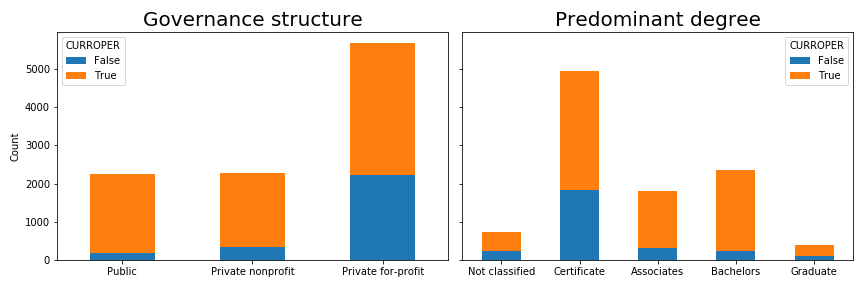
\includegraphics[width=4.25in]{currentGovDegStackBars.png}
\end{figure}
Distribution of schools in the data by governance (left), predominant degree (right), and whether they are currently operating (CURROPER).
\end{center}
\end{frame}
%------------------------------------------------
\begin{frame} 
\frametitle{Features of analyzed schools}
Public schools are larger and less expensive than private schools. Private non-profit schools are slightly larger and more expensive than private for-profit schools, though private for-profit schools show more variation in enrollment and cost than private nonprofit schools.

\begin{columns}
\column{2in}
\begin{figure}
\includegraphics[width=2in]{currentUGDSControlBox.png}
\end{figure}
\column{2in}
\begin{figure}
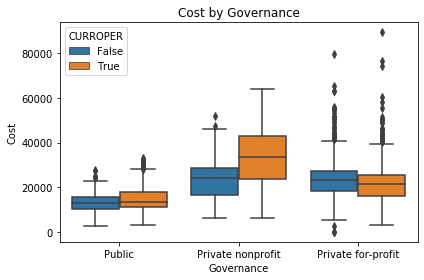
\includegraphics[width=2in]{currentCostGovBox.png}
\end{figure}
\end{columns}
\begin{center}
Enrollment (left) and cost (right) of schools by governance structure and whether they are currently operating (CURROPER).  \end{center}
\end{frame}
%------------------------------------------------
\begin{frame} 
\frametitle{Features of analyzed schools}
Private non-profit schools offer predominantly bachelor's degrees, and are more expensive. Public schools are less expensive than private for-profit schools for all degree types.

\begin{center}
\begin{figure}
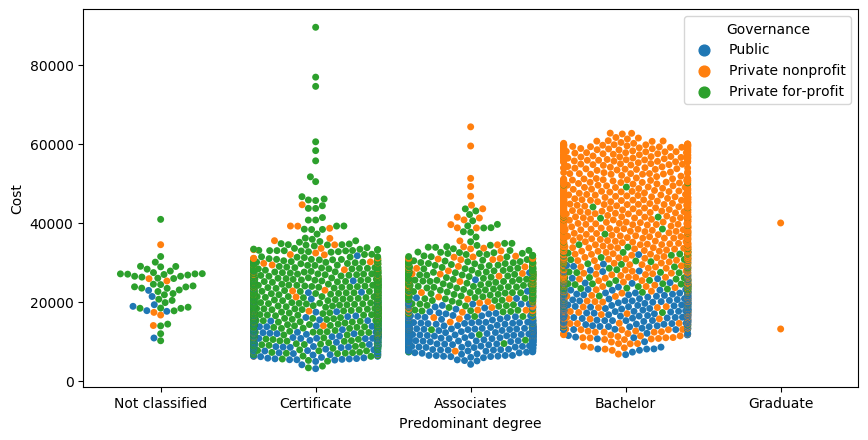
\includegraphics[width=4.25in]{currentPriceDegreeSwarm.png}
\end{figure}
Cost by degree type and governance structure.
\end{center}
\end{frame}
%------------------------------------------------
%\begin{frame} 
%\frametitle{Features of analyzed schools}
%\begin{center}
%\begin{figure}
%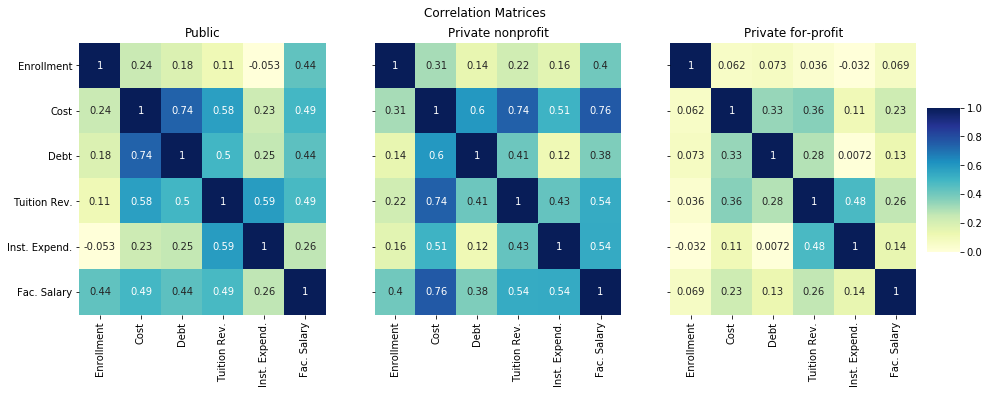
\includegraphics[width=4.25in]{currentFinanceCorrelationHeatmap.png}
%\end{figure}
%Pearson correlation coefficients for various financial metrics by school governance structure.
%\end{center}
%\end{frame}
%------------------------------------------------
%------------------------------------------------
\section{Recommendations and Key Findings} % 1 slide
%------------------------------------------------
\begin{frame}
\frametitle{Recommendations}
\begin{block}{Use model to predict status of member institutions.}
\begin{itemize}
\item Run 180+ member schools through model.
\item Pay attention to schools that are predicted to be 'closed'.
\end{itemize}
\end{block}

\begin{block}{Use model to predict probabilities of school closings.}
\begin{itemize}
\item Model generates probability that each school is open.
\item Current model uses 50\% as threshold.
\item Can adjust threshold for classification, or examine the probabilities.
\end{itemize}
\end{block}
\end{frame}

%------------------------------------------------
\section{Modeling Results and Analysis } % 3-4 slides
%------------------------------------------------
\begin{frame}
\frametitle{Data Processing}

\textbf{Impute} missing values using group median
\begin{itemize}
\item Institution name and federal ID
\item Governance structure  
\item Predominant degree 
\end{itemize}
\textbf{Filter} data by year
\begin{itemize}
\item Closed schools from 2010-2013
\item Currently operating schools from 2013
\end{itemize}

Double the number of minority class observations via \textbf{resampling} with replacement.

\vspace{1em}
12959 observations x 12 features

\end{frame}
%------------------------------------------------
\begin{frame}
\frametitle{Modeling}
\begin{enumerate}
\item Decision Tree model, which feeds 
\item AdaBoost model
\end{enumerate}

\begin{block} {AdaBoost Model Performance Metrics}
\begin{table}[h]
\begin{center}
\begin{tabular}{l l | c c r }
\multicolumn{2}{l}{Currently operating} & \multicolumn{2}{c}{Predicted} & Recall \\
& & No & Yes &  \\ 
\cline{2-5}
Actual & No & 1227 &  30 & 0.98 \\
& Yes & 69 & 2163 & .97 \\  \hline
Precision&  & .95 & .99 \\ 
Accuracy & & &  & .97 \\
	\end{tabular}
	\label{tab:ABConfusionNoDup}
	\caption{Confusion matrix and evaluation metrics for the final AdaBoost model with duplicated/resampled observations removed.}
\end{center}
\end{table}
\end{block}
\end{frame}

%------------------------------------------------
\begin{frame} 
\frametitle{Model results}
\begin{columns}
\column{2in}
\begin{figure}
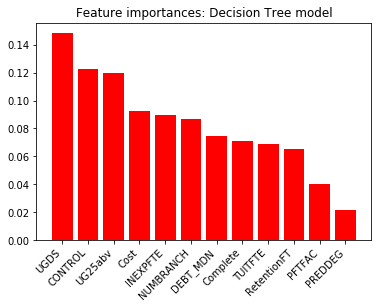
\includegraphics[width=2in]{DTFeatureImportance.png}
\end{figure}

\column{2in}
\begin{figure}
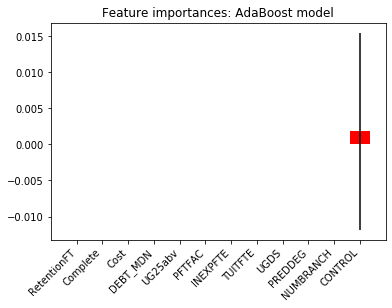
\includegraphics[width=2in]{ABFeatureImportance.png}
\end{figure}
\end{columns}
\begin{center}
Feature importance levels based on the Decision Tree model (left) and the AdaBoost model (right).
\end{center}
\end{frame}
%------------------------------------------------

\begin{frame}
\frametitle{Model results}

\begin{table}
\begin{tabularx}{4in}{l | L | c | L | c}
& \multicolumn{2}{c}{Decision Tree} & \multicolumn{2}{c}{AdaBoost} \\
& Factor & Coefficient & Factor & Coefficient \\ \hline
1 & Undergrad enrollment & 0.148392 & Governance structure & 0.001795 \\ \hline
2 & Governance structure & 0.122221 &  *All other features & null \\ \hline
3 &  \% students over age 25 & 0.119403 & & \\ \hline
4 & Cost & 0.092577 & & \\ \hline
5 & Instructional expenditure & 0.089737 & & \\ \hline
\end{tabularx}
\label{tab:features}
\caption{Top 5 predictive features and coefficients}
\end{table}
\end{frame}
%-----------------------------------------------
\begin{frame}
\frametitle{Nonprofit schools - Bachelor's degrees \newline
False negative results}

%\begin{footnotesize}
\begin{table}
\begin{tabularx}{4in}{L c c c c}
School & Predict & Probab & 2013 & 2020 \\ \hline
St. Andrews University & F &0.258114 & T & T \\ \hline
Central Methodist University - College of Graduate ... & F & 0.252362 & T & T \\ \hline
The Robert B Miller College & F & 0.440132 & T & F \\ \hline
\end{tabularx}
\end{table}
%\end{footnotesize}

\end{frame}
%------------------------------------------------
\begin{frame} 
\frametitle{Nonprofit schools \newline 
Predicted probability between 50-60\%}

\begin{footnotesize}
\begin{table}
\begin{tabularx}{4.5in}{L c c c c}

School & Predict & Probab & 2013 & 2020 \\ \hline
Rabbinical Seminary M'kor Chaim & T & 0.582 & F & No website \\ 
Remington College - Dallas & T & 0.585 & F & T ?\\
Florida Christian College & T & 0.535 & F & No website \\ 
ICC Technical Institute & T & 0.517 & F & No website\\ 
Remington College of Nursing - Orlando & T &  0.581  & T & Rename/merge \\
Alegent Creighton Health School of Radiologic... & T & 0.515 & T & Rename/merge \\
CET-Salinas & T & 0.531 & T & T \\
National University of Health Sciences & T & 0.506  & T & T \\
Baptist Missionary Association Theological Sem... & T &  0.582 & T & T \\
Universidad Teologica del Caribe & T &  0.544 & T & T \\
Annenberg School of Nursing & T & 0.520  & T & T \\

\end{tabularx}
\end{table}
%\normalsize
\end{footnotesize}

\end{frame}

%------------------------------------------------
\section{Summary \& Conclusions} % 1 slide
%------------------------------------------------
\subsection{Conclusions}
%------------------------------------------------
\begin{frame}{Conclusions}
\begin{itemize}

\item Private for-profit schools make up > 50\% of the schools in the data. While private for profit schools may be slightly more likely to be predicted as open, there are more closed for-profit schools in the database than other governance types.
\item Schools with more students may be more likely to stay open.
\end{itemize}

\textbf{Future directions}: Update the model with more recent data, other financial measures (e.g., endowment size, institutional debt, unfunded discount rate), and other data sources (e.g. US News \& World Report rankings).

\end{frame}
%------------------------------------------------
\end{document} 